\chapter{\hspace{2.6em} Uppgift för prototypning}
\label{cha:gruppens_skisser}

\section{Skissbas för prototypuppgift}
\label{sec:skissbas}
\begin{figure}[H]
  \centering
  \includegraphics[scale=0.33]{Skissbas}
  \caption{Skissbas gruppmedlemmarna var givna att utgå från för sin prototyp.}
  \label{fig:skissbas}
\end{figure}

\section{Prototypuppgift}
\label{sec:prototype-exercise}
På skissbasen (figur \ref{fig:skissbas}) ska du, på valfritt sätt (digitalt/analogt), rita en snabb skiss över hur du tänker att \textit{hjälpknappen och hjälprutan} ska se ut. Skissen ska vara tydlig, och du ska rita den så som du har föreställt dig den i huvudet när vi har pratat om den, och med så lite påverkan från andra som möjligt. 

\section{Gruppmedlemmars resultat av prototypuppgift}
\label{sec:gruppens_skisser}
\begin{figure}[!htb]
  \centering
  \includegraphics[scale=0.33]{pt_help_johan_n}
  \caption{Prototyp av gruppmedlem A gjord enligt uppgiften.}
  \label{fig:pt_help_johan_n}
\end{figure}
\ 
\begin{figure}[H]
  \centering
  \includegraphics[scale=0.33]{pt_help_johan_t}
  \caption{Prototyp av gruppmedlem B gjord enligt uppgiften.}
  \label{fig:pt_help_johan_t}
\end{figure}
\ 
\begin{figure}[H]
  \centering
  \includegraphics[scale=0.65]{pt_help_joakim}
  \caption{Prototyp av gruppmedlem C gjord enligt uppgiften.}
  \label{fig:pt_help_joakim}
\end{figure}
\ 
\begin{figure}[H]
  \centering
  \includegraphics[scale=0.55]{pt_help_sebastian}
  \caption{Prototyp av gruppmedlem D gjord enligt uppgiften.}
  \label{fig:pt_help_sebastian}
\end{figure}
\ 
\begin{figure}[H]
  \centering
  \includegraphics[scale=0.5]{pt_help_victor}
  \caption{Prototyp av gruppmedlem E gjord enligt uppgiften.}
  \label{fig:pt_help_victor}
\end{figure}
\ 
\begin{figure}[H]
  \centering
  \includegraphics[scale=0.33]{pt_help_daniel}
  \caption{Prototyp av gruppmedlem F gjord enligt uppgiften.}
  \label{fig:pt_help_daniel}
\end{figure}
\ 
\begin{figure}[H]
  \centering
  \includegraphics[scale=0.33]{help_6b66d882}
  \caption{Prototyp av gruppmedlem G gjord enligt uppgiften.}
  \label{fig:pt_help_jonathan}
\end{figure}
\ 

\chapter{\hspace{2.6em} Frågeformulär: Att arbeta med och utan prototyper}
\label{cha:prototyper_enkat}
\section{Frågeformulär: Att arbeta med och utan prototyper}
\label{sec:prototyper_enkat}
Frågorna i enkäten handlade om utseende hos olika features i applikationen. Alla frågor var obligatoriska utom den sista frågan som endast var ett fält för övriga kommentarer.

\subsection{Hjälpknapp och hjälpruta}
Fokusera på utseende och design av hjälpknapp och hjälpruta. Ignorera hur resten av användargränssnittet ser ut.
Din prototyp syftar på den prototyp som du fick rita ovanpå den avgivna skissbasen.

\begin{figure}[H]
  \centering
  \includegraphics[scale=0.33]{help_a8eb86d4}
  \label{fig:help_1}
  \caption{Hjälpknapp och hjälpruta, version 1}
\end{figure}
\ 

\begin{figure}[H]
  \centering
  \includegraphics[scale=0.8]{help_a8eb86d4_zoom}
  \label{fig:help_1_zoom}
  \caption{Förtydligande av hjälpknapp och hjälpruta, version 1}
\end{figure}

\begin{table}[h!]
  \caption{Frågor om hjälpknapp och hjälpruta, version 1}
  \def\arraystretch{1.5}
  \begin{adjustbox}{max width=\textwidth}
    \begin{tabularx}{\textwidth}{ | c | X | r |}
      \hline
      \textbf{Nr} & \textbf{Fråga} & \textbf{Svarstyp} \\
      \hline
      1.1 & Hur väl stämmer detta resultat överens med din prototyp? & Skala 1-5 \\
      \hline
      1.2 & Hur nöjd är du med detta resultat? & Skala 1-5 \\
      \hline 
    \end{tabularx}
  \end{adjustbox}
  \label{tab:prototyp_enkat_help_1}
\end{table}
\ 

\begin{figure}[H]
  \centering
  \includegraphics[scale=0.33]{help_eb750c41}
  \label{fig:help_2}
  \caption{Hjälpknapp och hjälpruta, version 2}
\end{figure}
\ 

\begin{figure}[H]
  \centering
  \includegraphics[scale=0.7]{help_eb750c41_zoom}
  \label{fig:help_2_zoom}
  \caption{Förtydligande av hjälpknapp och hjälpruta, version 2}
\end{figure}
\ 

\begin{table}[h!]
  \caption{Frågor om hjälpknapp och hjälpruta, version 2}
  \def\arraystretch{1.5}
  \begin{adjustbox}{max width=\textwidth}
    \begin{tabularx}{\textwidth}{ | c | X | r |}
      \hline
      \textbf{Nr} & \textbf{Fråga} & \textbf{Svarstyp} \\
      \hline
      2.1 & Hur väl stämmer detta resultat överens med din prototyp? & Skala 1-5 \\
      \hline
      2.2 & Hur nöjd är du med detta resultat? & Skala 1-5 \\
      \hline 
    \end{tabularx}
  \end{adjustbox}
  \label{tab:prototyp_enkat_help_2}
\end{table}
\ 

\begin{figure}[H]
  \centering
  \includegraphics[scale=0.33]{help_6b66d882}
  \label{fig:help_3}
  \caption{Hjälpknapp och hjälpruta, version 3}
\end{figure}
\ 

\begin{figure}[H]
  \centering
  \includegraphics[scale=0.65]{help_6b66d882_zoom}
  \label{fig:help_3_zoom}
  \caption{Förtydligande av hjälpknapp och hjälpruta, version 3}
\end{figure}
\ 

\begin{table}[h!]
  \caption{Frågor om hjälpknapp och hjälpruta, version 3}
  \def\arraystretch{1.5}
  \begin{adjustbox}{max width=\textwidth}
    \begin{tabularx}{\textwidth}{ | c | X | r |}
      \hline
      \textbf{Nr} & \textbf{Fråga} & \textbf{Svarstyp} \\
      \hline
      3.1 & Hur väl stämmer detta resultat överens med din prototyp? & Skala 1-5 \\
      \hline
      3.2 & Hur nöjd är du med detta resultat? & Skala 1-5 \\
      \hline 
    \end{tabularx}
  \end{adjustbox}
  \label{tab:prototyp_enkat_help_3}
\end{table}
\ 

\subsection{Tabell i den detaljerade vyn}
Fokusera på utseende och design av tabell för den detaljerade vyn. Ignorera innehållet i cellerna och hur resten av användargränssnittet ser ut.
För följande avsnitt ska du jämföra kommande alternativ med nedanstående prototyp.

\begin{figure}[H]
  \centering
  \includegraphics[scale=0.5]{table_prototype}
  \caption{Prototyp för tabellen i den detaljerade vyn skapad av gruppen under förstudien.}
  \label{fig:table_0}
\end{figure}
\

\begin{table}[h!]
  \caption{Frågor om prototyp för tabellen i den detaljerade vyn.}
  \def\arraystretch{1.5}
  \begin{adjustbox}{max width=\textwidth}
    \begin{tabularx}{\textwidth}{ | c | X | r |}
      \hline
      \textbf{Nr} & \textbf{Fråga} & \textbf{Svarstyp} \\
      \hline
      4.1 & Hur väl stämmer prototypen överens med din initiala bild av tabellen? & Skala 1-5 \\
      \hline
      4.2 & Hur nöjd är du med tabellens utseende i denna prototyp? & Skala 1-5 \\
      \hline 
    \end{tabularx}
  \end{adjustbox}
  \label{tab:prototyp_enkat_table_0}
\end{table}
\ 

\begin{figure}[H]
  \centering
  \includegraphics[scale=0.34]{table_eb750c41}
  \label{fig:table_1}
  \caption{Tabellen i den detaljerade vyn, version 1.}
\end{figure}
\ 

\begin{table}[h!]
  \caption{Frågor om tabellen i den detaljerade vyn, version 1.}
  \def\arraystretch{1.5}
  \begin{adjustbox}{max width=\textwidth}
    \begin{tabularx}{\textwidth}{ | c | X | r |}
      \hline
      \textbf{Nr} & \textbf{Fråga} & \textbf{Svarstyp} \\
      \hline
      5.1 & Hur väl stämmer detta resultat överens med din prototyp? & Skala 1-5 \\
      \hline
      5.2 & Hur nöjd är du med detta resultat? & Skala 1-5 \\
      \hline 
    \end{tabularx}
  \end{adjustbox}
  \label{tab:prototyp_enkat_table_1}
\end{table}
\ 

\begin{figure}[H]
  \centering
  \includegraphics[scale=0.33]{table_6b66d882}
  \label{fig:table_2}
  \caption{Tabellen i den detaljerade vyn, version 2.}
\end{figure}
\ 

\begin{table}[h!]
  \caption{Frågor om tabellen i den detaljerade vyn, version 2.}
  \def\arraystretch{1.5}
  \begin{adjustbox}{max width=\textwidth}
    \begin{tabularx}{\textwidth}{ | c | X | r |}
      \hline
      \textbf{Nr} & \textbf{Fråga} & \textbf{Svarstyp} \\
      \hline
      6.1 & Hur väl stämmer detta resultat överens med din prototyp? & Skala 1-5 \\
      \hline
      6.2 & Hur nöjd är du med detta resultat? & Skala 1-5 \\
      \hline 
    \end{tabularx}
  \end{adjustbox}
  \label{tab:prototyp_enkat_table_2}
\end{table}
\ 
\newpage
\subsection{Avslutande frågor}
\begin{table}[h!]
  \caption{Frågor som ställdes sist i enkäten.}
  \def\arraystretch{1.5}
  \begin{adjustbox}{max width=\textwidth}
    \begin{tabularx}{\textwidth}{ | c | X | r |}
      \hline
      \textbf{Nr} & \textbf{Fråga} & \textbf{Svarstyp} \\
      \hline
      7.1 & Upplever du att du har fått göra om features för att resultatets utseende inte stämde överens med andra gruppmedlemmars bild av det? & Ja/Nej \\
      \hline
      7.2 & Tycker du att det har underlättat utvecklingen att ha prototyper att jobba efter? & Skala 1-5 \\
      \hline 
      7.3 & På vilket/vilka sätt har det underlättat/inte underlättat? & Fritext \\
      \hline 
      7.4 & Tycker du att tiden som spenderats på att ta fram prototyper har varit väl spenderad tid? & Skala 1-5 \\
      \hline 
      7.5 & Hade du velat att gruppen hade tagit fram prototyper för fler features? & Ja, fler/Nej, lagom många/Nej, färre \\
      \hline 
      7.6 & Hade du velat att gruppen hade utvecklat de existerande prototyperna mer? & Ja, mer/Nej, lagom/Nej, mindre \\
      \hline 
      7.7 & Kommentarer & Fritext \\
      \hline  
    \end{tabularx}
  \end{adjustbox}
  \label{tab:prototyp_enkat_last_questions}
\end{table}
\ 

%*****************************************
%*************** RESULTAT ****************
%*****************************************
\chapter{\hspace{2.6em} Resultat från frågeformulär om prototyper}
\label{cha:prototyper_enkat_resultat}
\section{Resultat från enkät om prototyper}
\label{sec:prototyper_enkat_resultat}

\subsection{Hjälpknapp och hjälpruta}
\begin{figure}[H]
	\centering
	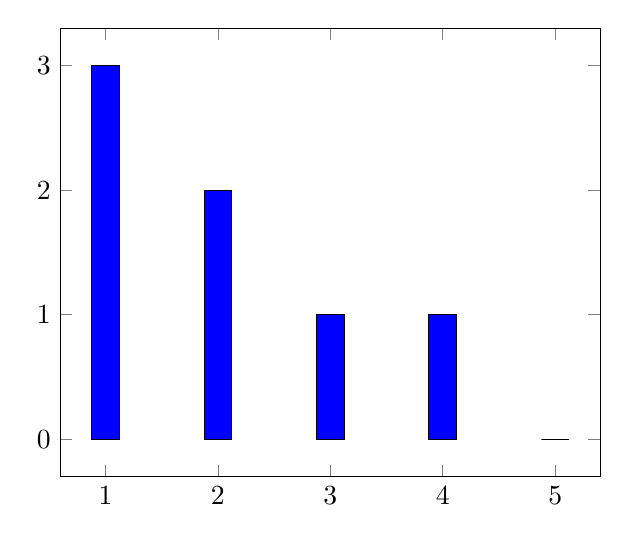
\begin{tikzpicture}
	%\label{bar:results_first}
		\begin{axis}[
			symbolic x coords={1, 2, 3, 4, 5},
			xtick=data
			]
			\addplot[ybar,fill=blue] coordinates {
				(1,  3)
				(2,  2)
				(3,  1)
				(4,  1)
				(5,  0)
			};
		\end{axis}
	\end{tikzpicture}
	\caption{Fråga 1.1: Hur väl stämmer hjälprutan version 1 överens med din prototyp?}
\end{figure}

\begin{figure}[H]
  \centering
  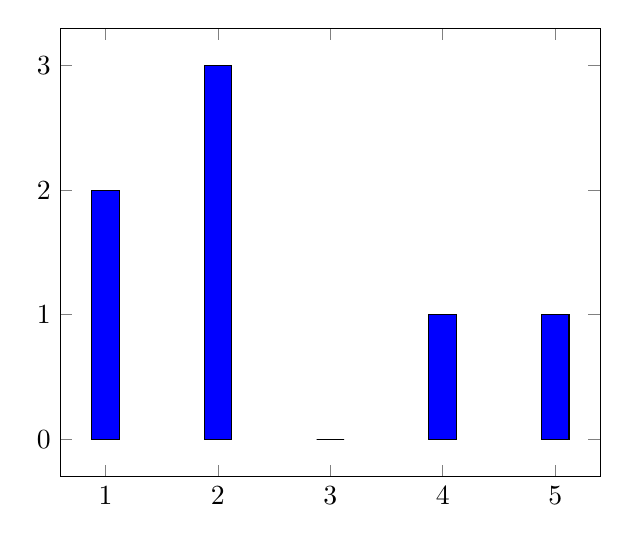
\begin{tikzpicture}
  %\label{bar:results_first}
    \begin{axis}[
      symbolic x coords={1, 2, 3, 4, 5},
      xtick=data
      ]
      \addplot[ybar,fill=blue] coordinates {
        (1,  2)
        (2,  3)
        (3,  0)
        (4,  1)
        (5,  1)
      };
    \end{axis}
  \end{tikzpicture}
  \caption{Fråga 1.2: Hur nöjd är du med resultatet i hjälprutan version 1?}
\end{figure}

\begin{figure}[H]
  \centering
  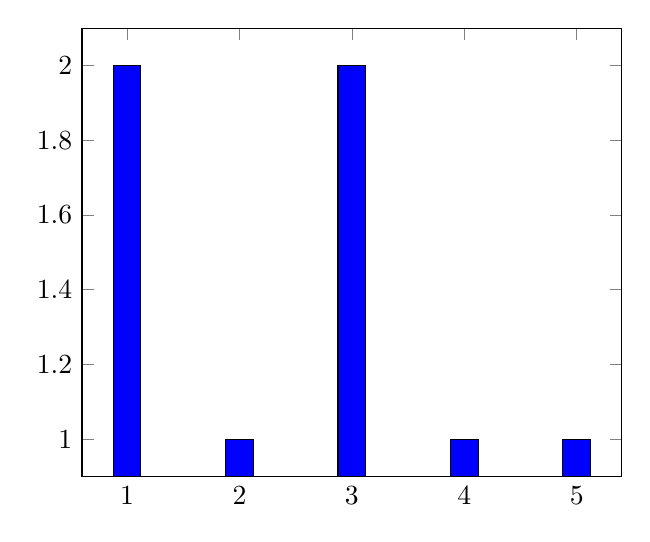
\begin{tikzpicture}
  %\label{bar:results_first}
    \begin{axis}[
      symbolic x coords={1, 2, 3, 4, 5},
      xtick=data
      ]
      \addplot[ybar,fill=blue] coordinates {
        (1,  2)
        (2,  1)
        (3,  2)
        (4,  1)
        (5,  1)
      };
    \end{axis}
  \end{tikzpicture}
  \caption{Fråga 2.1: Hur väl stämmer hjälprutan version 2 överens med din prototyp?}
\end{figure}

\begin{figure}[H]
  \centering
  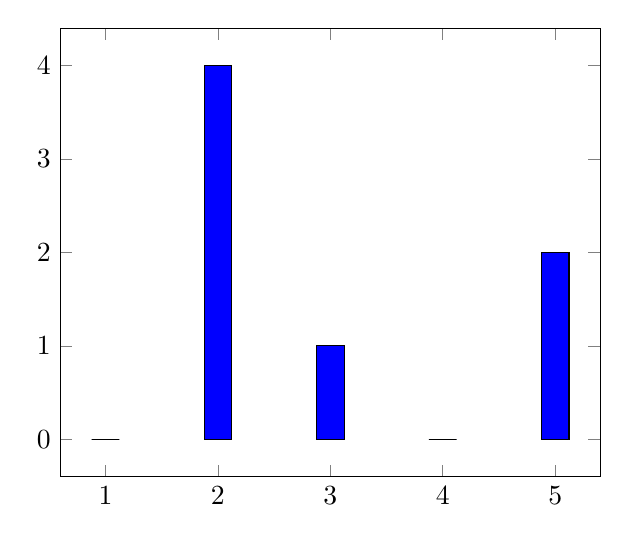
\begin{tikzpicture}
  %\label{bar:results_first}
    \begin{axis}[
      symbolic x coords={1, 2, 3, 4, 5},
      xtick=data
      ]
      \addplot[ybar,fill=blue] coordinates {
        (1,  0)
        (2,  4)
        (3,  1)
        (4,  0)
        (5,  2)
      };
    \end{axis}
  \end{tikzpicture}
  \caption{Fråga 2.2: Hur nöjd är du med resultatet i hjälprutan version 2?}
\end{figure}

\begin{figure}[H]
  \centering
  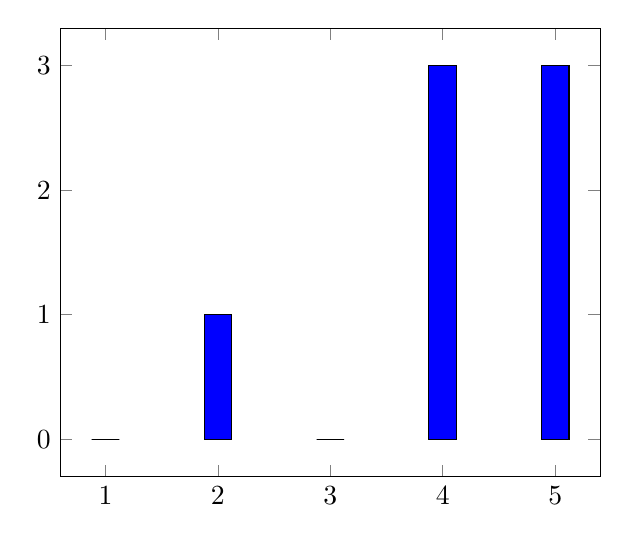
\begin{tikzpicture}
  %\label{bar:results_first}
    \begin{axis}[
      symbolic x coords={1, 2, 3, 4, 5},
      xtick=data
      ]
      \addplot[ybar,fill=blue] coordinates {
        (1,  0)
        (2,  1)
        (3,  0)
        (4,  3)
        (5,  3)
      };
    \end{axis}
  \end{tikzpicture}
  \caption{Fråga 3.1: Hur väl stämmer hjälprutan version 3 överens med din prototyp?}
\end{figure}

\begin{figure}[H]
  \centering
  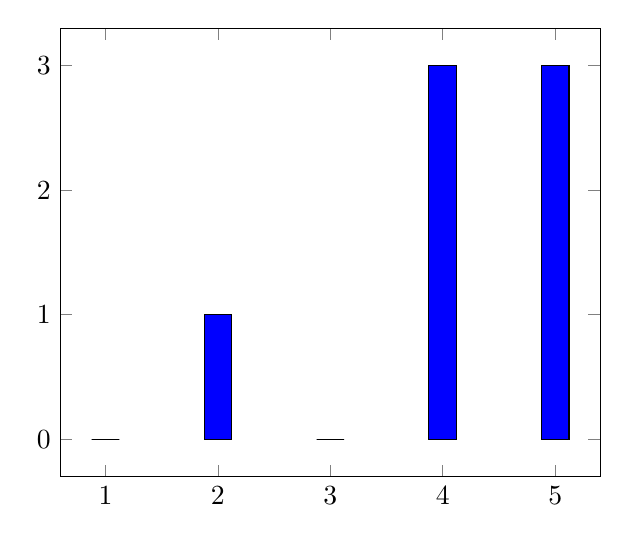
\begin{tikzpicture}
  %\label{bar:results_first}
    \begin{axis}[
      symbolic x coords={1, 2, 3, 4, 5},
      xtick=data
      ]
      \addplot[ybar,fill=blue] coordinates {
        (1,  0)
        (2,  1)
        (3,  0)
        (4,  3)
        (5,  3)
      };
    \end{axis}
  \end{tikzpicture}
  \caption{Fråga 3.2: Hur nöjd är du med resultatet i hjälprutan version 3?}
\end{figure}

\subsection{Tabellen i den detaljerade vyn}
\begin{figure}[H]
  \centering
  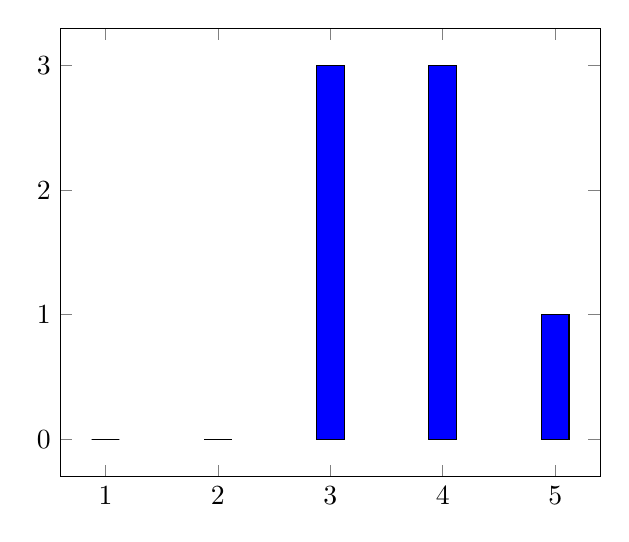
\begin{tikzpicture}
  %\label{bar:results_first}
    \begin{axis}[
      symbolic x coords={1, 2, 3, 4, 5},
      xtick=data
      ]
      \addplot[ybar,fill=blue] coordinates {
        (1,  0)
        (2,  0)
        (3,  3)
        (4,  3)
        (5,  1)
      };
    \end{axis}
  \end{tikzpicture}
  \caption{Fråga 4.1: Hur väl stämmer prototypen överens med din initiala bild av prototypens utseende?}
\end{figure}

\begin{figure}[H]
  \centering
  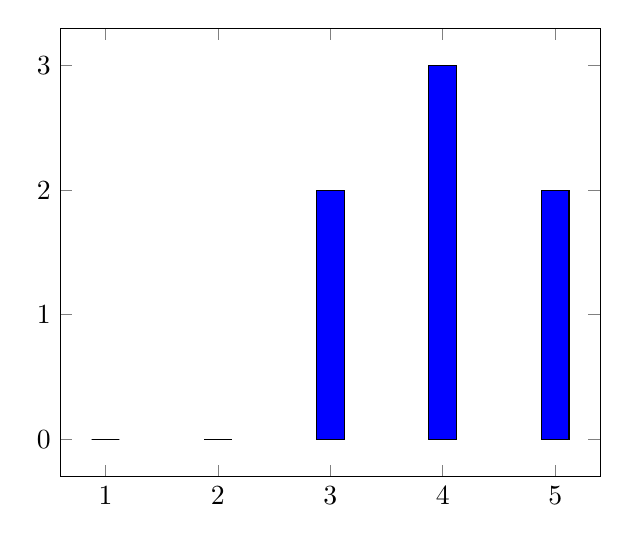
\begin{tikzpicture}
  %\label{bar:results_first}
    \begin{axis}[
      symbolic x coords={1, 2, 3, 4, 5},
      xtick=data
      ]
      \addplot[ybar,fill=blue] coordinates {
        (1,  0)
        (2,  0)
        (3,  2)
        (4,  3)
        (5,  2)
      };
    \end{axis}
  \end{tikzpicture}
  \caption{Fråga 4.2: Hur nöjd är du med tabellens utseende i denna prototyp?}
\end{figure}

\begin{figure}[H]
  \centering
  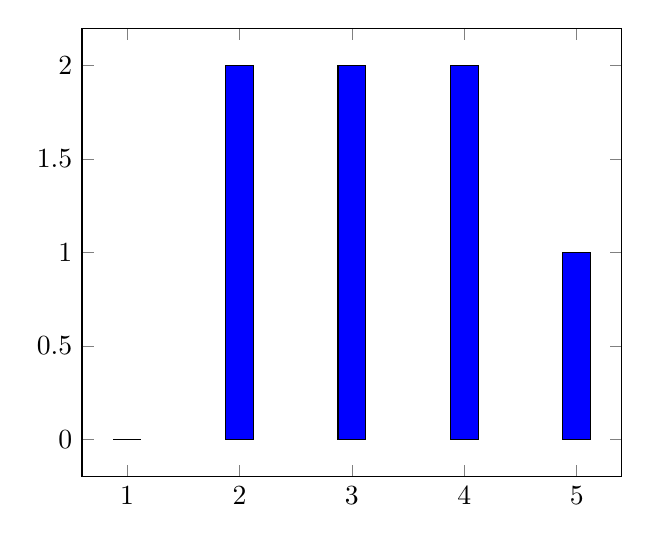
\begin{tikzpicture}
  %\label{bar:results_first}
    \begin{axis}[
      symbolic x coords={1, 2, 3, 4, 5},
      xtick=data
      ]
      \addplot[ybar,fill=blue] coordinates {
        (1,  0)
        (2,  2)
        (3,  2)
        (4,  2)
        (5,  1)
      };
    \end{axis}
  \end{tikzpicture}
  \caption{Fråga 5.1: Hur väl stämmer tabellen version 1 överens med gruppens prototyp?}
\end{figure}

\begin{figure}[H]
  \centering
  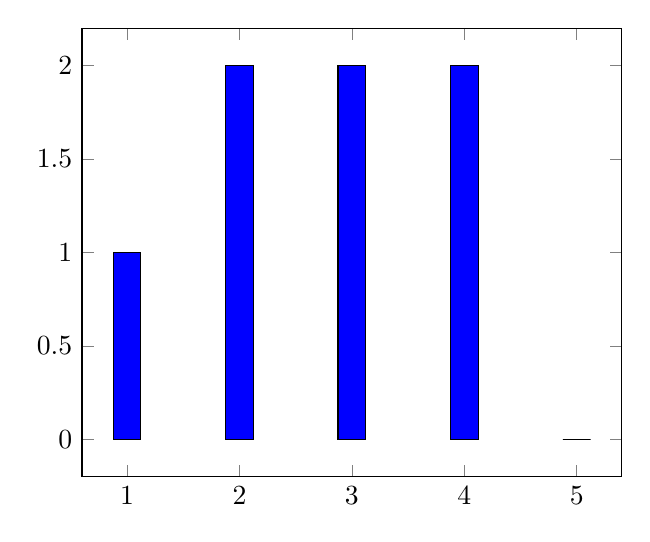
\begin{tikzpicture}
  %\label{bar:results_first}
    \begin{axis}[
      symbolic x coords={1, 2, 3, 4, 5},
      xtick=data
      ]
      \addplot[ybar,fill=blue] coordinates {
        (1,  1)
        (2,  2)
        (3,  2)
        (4,  2)
        (5,  0)
      };
    \end{axis}
  \end{tikzpicture}
  \caption{Fråga 5.2: Hur nöjd är du med resultatet i tabellen version 1?}
\end{figure}

\begin{figure}[H]
  \centering
  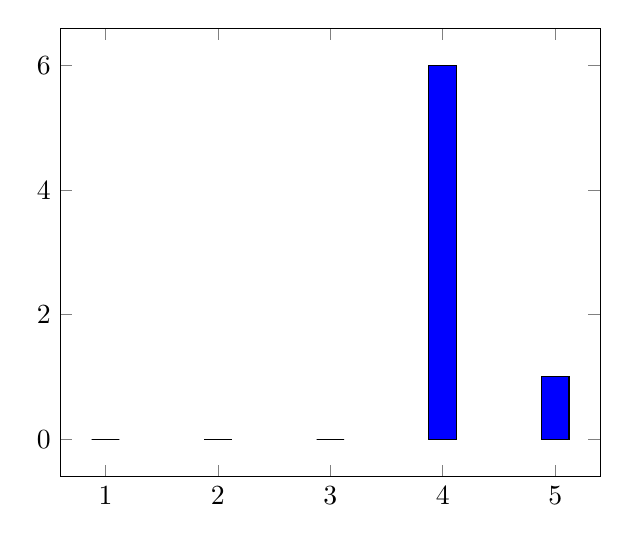
\begin{tikzpicture}
  %\label{bar:results_first}
    \begin{axis}[
      symbolic x coords={1, 2, 3, 4, 5},
      xtick=data
      ]
      \addplot[ybar,fill=blue] coordinates {
        (1,  0)
        (2,  0)
        (3,  0)
        (4,  6)
        (5,  1)
      };
    \end{axis}
  \end{tikzpicture}
  \caption{Fråga 6.1: Hur väl stämmer tabellen version 2 överens med gruppens prototyp?}
\end{figure}

\begin{figure}[H]
  \centering
  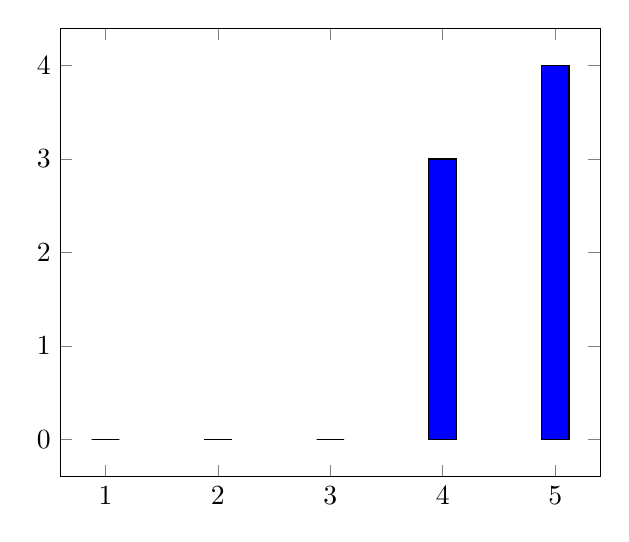
\begin{tikzpicture}
  %\label{bar:results_first}
    \begin{axis}[
      symbolic x coords={1, 2, 3, 4, 5},
      xtick=data
      ]
      \addplot[ybar,fill=blue] coordinates {
        (1,  0)
        (2,  0)
        (3,  0)
        (4,  3)
        (5,  4)
      };
    \end{axis}
  \end{tikzpicture}
  \caption{Fråga 6.2: Hur nöjd är du med resultatet i tabellen version 2?}
\end{figure}

\subsection{Avslutande frågor}
\begin{figure}[H]
  \centering
  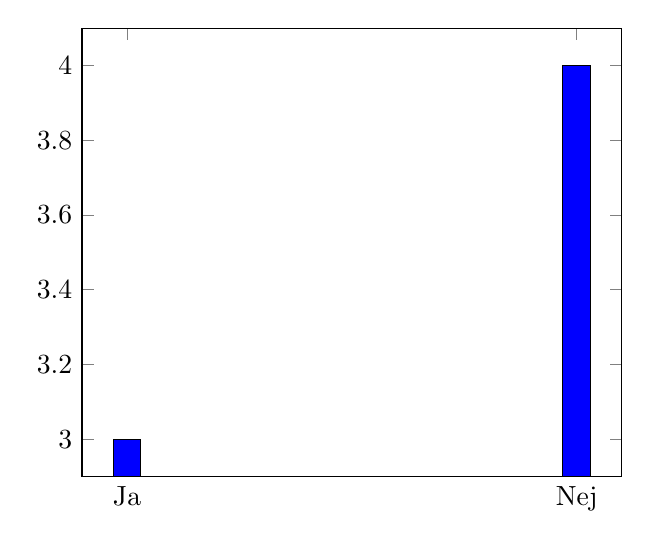
\begin{tikzpicture}
  %\label{bar:results_first}
    \begin{axis}[
      symbolic x coords={Ja, Nej},
      xtick=data
      ]
      \addplot[ybar,fill=blue] coordinates {
        (Ja,   3)
        (Nej,  4)
      };
    \end{axis}
  \end{tikzpicture}
  \caption{Fråga 7.1: Upplever du att du har fått göra om features för att resultatets utseende inte stämde överens med andra gruppmedlemmars bild av det?}
\end{figure}

\begin{figure}[H]
  \centering
  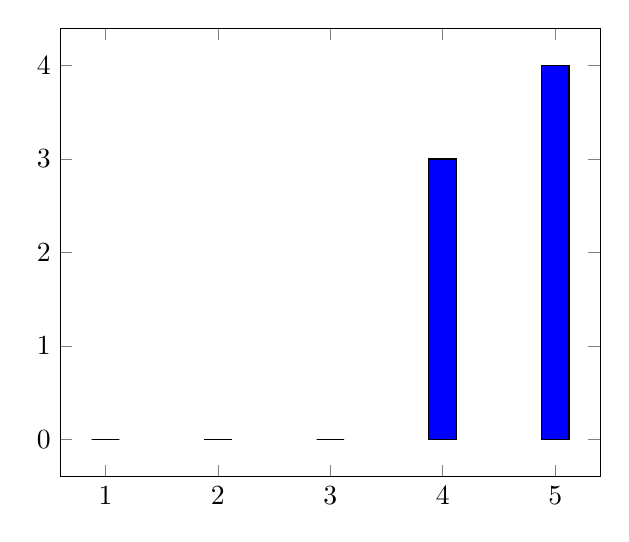
\begin{tikzpicture}
  %\label{bar:results_first}
    \begin{axis}[
      symbolic x coords={1, 2, 3, 4, 5},
      xtick=data
      ]
      \addplot[ybar,fill=blue] coordinates {
        (1,  0)
        (2,  0)
        (3,  0)
        (4,  3)
        (5,  4)
      };
    \end{axis}
  \end{tikzpicture}
  \caption{Fråga 7.2: Tycker du att det har underlättat utvecklingen att jobba med prototyper?}
\end{figure}

\begin{table}[h!]
  \caption{Fråga 7.3: På vilket/vilka sätt har det underlättat/inte underlättat?}
  \def\arraystretch{1.5}
  \begin{adjustbox}{max width=\textwidth}
    \begin{tabularx}{\textwidth}{ | X |}
      \hline
      \textbf{Svar} \\
      \hline
      Man får mindre iterationer om man följer en specad standard då personer får vara nöjda när den är uppnådd. \\
      \hline
      Det ger en målbild att jobba mot och något som kan användas som diskussionsunderlag för hur resten av prototypandet ska fortsätta \\
      \hline
      Man får en tydlig bild av hur slutresultat förväntas se ut. \\
      \hline 
      Som en tydlig kravspec att följa \\
      \hline 
      Många designbeslut finns tydligt visualiserade och det behövdes för att man skulle veta hur feature'n skulle anpassas. \\
      \hline 
      Lättare att ha gemensam bild av vad som ska göras. \\
      \hline 
      En bra startbild \\
      \hline  
    \end{tabularx}
  \end{adjustbox}
  \label{tab:prototyp_enkat_ease}
\end{table}

\begin{figure}[H]
  \centering
  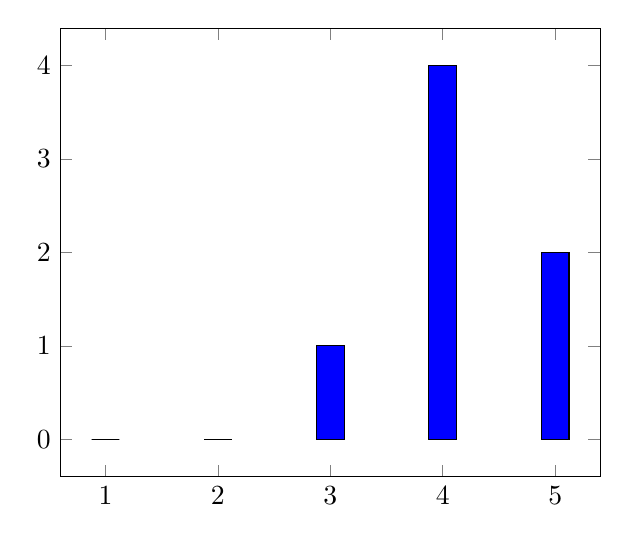
\begin{tikzpicture}
  %\label{bar:results_first}
    \begin{axis}[
      symbolic x coords={1, 2, 3, 4, 5},
      xtick=data
      ]
      \addplot[ybar,fill=blue] coordinates {
        (1,  0)
        (2,  0)
        (3,  1)
        (4,  4)
        (5,  2)
      };
    \end{axis}
  \end{tikzpicture}
  \caption{Fråga 7.4: Tycker du att tiden som spenderats på att ta fram prototyper har varit väl spenderad tid?}
\end{figure}

\begin{figure}[H]
  \centering
  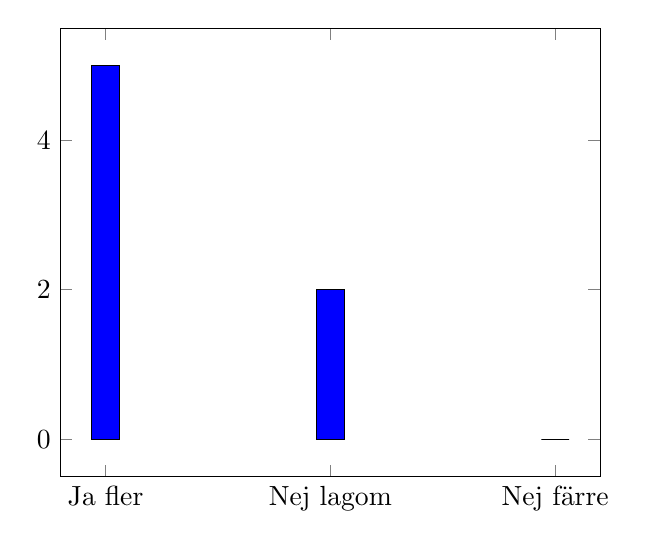
\begin{tikzpicture}
  %\label{bar:results_first}
    \begin{axis}[
      symbolic x coords={Ja fler, Nej lagom, Nej färre},
      xtick=data
      ]
      \addplot[ybar,fill=blue] coordinates {
        (Ja fler,    5)
        (Nej lagom,  2)
        (Nej färre,  0)
      };
    \end{axis}
  \end{tikzpicture}
  \caption{Fråga 7.5: Hade du velat att gruppen hade tagit fram prototyper för fler features?}
\end{figure}

\begin{figure}[H]
  \centering
  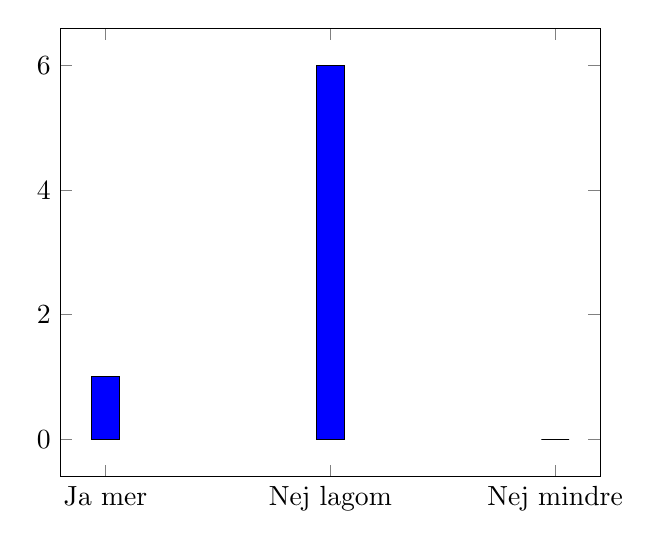
\begin{tikzpicture}
  %\label{bar:results_first}
    \begin{axis}[
      symbolic x coords={Ja mer, Nej lagom, Nej mindre},
      xtick=data
      ]
      \addplot[ybar,fill=blue] coordinates {
        (Ja mer,     1)
        (Nej lagom,  6)
        (Nej mindre, 0)
      };
    \end{axis}
  \end{tikzpicture}
  \caption{Fråga 7.6: Hade du velat att gruppen hade utvecklat de existerande prototyperna mer?}
\end{figure}

\begin{table}[h!]
  \caption{Fråga 7.7: Kommentarer (frivillig)}
  \def\arraystretch{1.5}
  \begin{adjustbox}{max width=\textwidth}
    \begin{tabularx}{\textwidth}{ | X |}
      \hline
      \textbf{Svar} \\
      \hline
      Prototyper är ett bra verktyg så att gruppen kan få en enhetlig bild av vad målet ska bli \\
      \hline
      Skönt att andra säger hur de vill ha det så man får flera perspektiv \\
      \hline  
    \end{tabularx}
  \end{adjustbox}
  \label{tab:prototyp_enkat_comments
}
\end{table}